\subsection{Testen von Web-Applikationen}
%Die Integration des Testens in die Software-Entwicklung ist auch bei
%Web-Applikationen sehr zu empfehlen. Modifikationen und Erweiterungen können
%so einfacher durchgeführt werden, da man weniger Gefahr läuft, dass als Folge
%davon plötzlich unerwartete Störungen auftreten. Ein gut konfiguriertes
%Testsystem ist in der Lage derartige Probleme frühzeitig aufzudecken.
%
%\newslide
Für das automatisierte Testen von Web-Applikationen
stehen eine Reihe frei-erhältlicher Tools zur Verfügung:
\begin{itemize}
%\item Cactus: das Test-Framework des Apache-Jakarta-Projektes für Unit-Tests
%  von server-seitigem Code (Servlets, Filters, Tag Libs, EJB \ldots)
%\href{http://jakarta.apache.org/cactus}{jakarta.apache.org/cactus}
\item HtmlUnit: automatisierter Funkionstest von Web-Seiten mit JavaScript,
  Cookies, Authentication und Page Redirection
\href{http://htmlunit.sourceforge.net/}{htmlunit.sourceforge.net}
\item JWebUnit: Durchführung von Abnahmetests
\href{http://jwebunit.sourceforge.net/}{jwebunit.sourceforge.net/}
\item MaxQ: Python-basiertes Aufnahme/Wiedergabe-Tool
\href{http://maxq.tigris.org/}{maxq.tigris.org/}
\item Canoo WebTest:

\href{http://webtest.canoo.com/webtest/manual/WebTestHome.html}
{webtest.canoo.com/webtest/manual/WebTestHome.html}
\item Selenium:
\href{http://selenium.openqa.org}{selenium.openqa.org}
\item Cargo: ein Wrapper für Java-EE-Container
 \href{http://cargo.codehaus.org/Home}{cargo.codehaus.org/Home}
\item JMeter: Durchführung von Lasttests
\href{http://jakarta.apache.org/jmeter}{jakarta.apache.org/jmeter}
\item Grinder: Durchführung von Lasttests mit Jython-Scripts
  \href{http://grinder.sourceforge.net}{grinder.sourceforge.net}
\end{itemize}
\newslide
\subsubsection{HtmlUnit}
HtmlUnit wird als ``Browser für Java-Programme'' bezeichnet.
HtmlUnit basiert auf Junit. Das heisst, man geht grundsätzlich wie gewohnt vor:
Man erstellt eine Testklasse und fügt
 dieser Klasse
 sukzessive die entsprechenden Testmethoden hinzu. 

\newslide
Am einfachsten verwendet man 
HtmlUnit mit Maven und ergänzt das POM-File mit folgendem Element:
\begin{lstlisting}[language=xml,
   morekeywords={dependency,groupId,artifactId,version,scope}]
<dependency>
  <groupId>net.sourceforge.htmlunit</groupId>
  <artifactId>htmlunit</artifactId>
  <version>2.4</version>
</dependency>
\end{lstlisting}
Dazu muss die Junit-Version auf den Wert 4.4 gesetzt werden.
\newslide
Als Testfall 
wird man in der Regel eine Server-Verbindung kreieren und überprüfen, ob die
erwarteten Ergebnisse zurückgegeben werden:
\begin{lstlisting}[language=java]
public class SimpleWebTest {
  @Test
  public void homePage() throws Exception {
    final WebClient webClient = new WebClient();
    final HtmlPage page = (HtmlPage)webClient.
                 getPage("http://localhost:8080/hitchhikers-guide");
    assertEquals("Welcome", page.getTitleText());
  }
\end{lstlisting}
\newslide
Das folgende Beispiel zeigt, dass auch Web-Formulare getestet werden können:
\begin{lstlisting}[language=java]
  @Test
  public void submitForm() throws Exception {
    final WebClient webClient = new WebClient();
    final HtmlPage page1 = (HtmlPage)webClient.
                 getPage("http://localhost:8080/hello/login");
    final HtmlForm page1.getFormByName("loginform");
    final HtmlTextInput textfield = form.getInputByName("username");
    final HtmlSubmitInput button = form.getInputByName("submit");

    textfield.setValueAttribute("douglas");
    final HtmlPage page2=(HtmlPage)button.click();
    assertEquals( "Main", page.getTitleText() );
  }
\end{lstlisting}

\newslide
\subsubsection{JWebUnit}
JWebUnit ist ein auf Junit und HtmlUnit basierendes
Java-Test-Framework für Web-Applikationen. JWebUnit verwendet man am
einfachsten mit Maven:
\begin{lstlisting}[language=xml,
  morekeywords={dependency,groupId,artifactId,version,scope}]
<dependency>
  <groupId>net.sourceforge.jwebunit</groupId>
  <artifactId>jwebunit-htmlunit-plugin</artifactId>
  <version>2.2</version>
  <scope>test</scope>
</dependency>
 \end{lstlisting}
\newslide
Im Vergleich zu HtmlUnit ist die Verwendung einfacher:
\begin{lstlisting}[language=java]
public class SimpleWebUnitWebTest extends WebTestCase {
  public void setUp(){
    getTestContext().
         setBaseUrl("http://localhost:8080/hitchhiker");
  }
  public void testHomePage() {
    beginAt("/");
    assertTitleEquals("Welcome");
  }
}
\end{lstlisting}
\newslide
Das gilt auch für Formulare:
\begin{lstlisting}[language=java]

  public void testSubmitForm() throws Exception {
    beginAt("/hello/login");
    assertFormPresent("loginform");
    assertFormElementPresent("username");
    setTextField("username", "douglas");
    submit();
    assertTitleEquals( "Main" );
  }
\end{lstlisting}
\newslide
Weitere Vereinfachungen betreffen das Testen von Tabellen und HTML-Elementen
und das Navigieren durch die Seiten.
\begin{lstlisting}[language=java]
  assertElementPresent("pageTitle");
  assertTextInElement("pageTitle", "Hello World");
\end{lstlisting}
In diesem Beispiel wird geprüft, ob ein Element
mit dem Id-Attribut ``pageTitle'' existiert und ob darin der
Text ``Hello World'' enthalten ist.

\newslide
Störend ist hier wie schon bei HtmlUnit, 
dass zuerst ein WebContainer gestartet
werden muss, bevor man die Tests durchführt.

\newslide
Dank Jetty können diese Tests aber wie normale Unit-Tests durchgeführt
werden:
\begin{lstlisting}[language=java]
import org.mortbay.jetty.Server;
public class SimpleWebUnitWebTest extends WebTestCase {
  private Server server;
	
  public void setUp() throws Exception{
    String context="/hitchhiker";
    // Port 0 means "assign arbitrarily port number"
    server = new Server(0);
    server.addHandler(new WebAppContext("src/main/webapp", context));
    server.start();
    int port = server.getConnectors()[0].getLocalPort();
    getTestContext().setBaseUrl("http://localhost:"+port+context);
  }
..
}
\end{lstlisting}
\newslide
Dazu muss lediglich die POM-Datei etwas angepasst werden:
\begin{lstlisting}[language=xml,
  morekeywords={dependency,groupId,artifactId,version,scope}]
    <dependency>
      <groupId>org.mortbay.jetty</groupId>
      <artifactId>jetty</artifactId>
      <version>6.1.14</version>
      <scope>test</scope>
    </dependency>
    <dependency>
      <groupId>org.mortbay.jetty</groupId>
      <artifactId>jsp-2.1</artifactId>
      <version>6.1.14</version>
      <scope>test</scope>
    </dependency> 
\end{lstlisting}
\newslide
% http://blog.bemoko.com/2009/07/01/automated-mobile-web-testing-with-canoo-webtest-were-impressed/
%
\subsubsection{Canoo WebTest}
Auch Canoo WebTest ist ein auf HtmlUnit basierendes
Java-Test-Framework für Web-Applikationen. Im Gegensatz zu JWebUnit
werden die Testfälle jedoch als Ant-Tasks definiert:
\begin{lstlisting}[language=xml,
  morekeywords={project,property,import,target,webtest,config,steps,invoke,verifyTitle,setInputField,clickButton,verifyTitle}]
<project name="SimpleTest" basedir="." default="wt.full">

  <property name="webtest.home"
            location="/usr/local/java/webtest-3.0" />
  <import file="${webtest.home}/webtest.xml"/>

    <!-- runs start page test -->
    <target name="wt.testInWork"
        description="executes start page test case">

      <webtest
         name="check that WebTest is Google's top result">
	<config summary="true" />
	<steps>
	  <invoke url="http://www.google.com/ncr"
		  description="Go to Google (in English)"/>
	  <verifyTitle text="Google" />
	  <setInputField name="q" value="WebTest" />
	  <clickButton label="I'm Feeling Lucky" />
	  <verifyTitle text="Canoo WebTest Homepage" />
	</steps>
      </webtest>
    </target>
</project>
\end{lstlisting}
Ausgeführt werden diese Tests mit der Anweisung:
\begin{lstlisting}
  webtest -f web-test.xml
\end{lstlisting}
Webtest ist auch in der Lage übersichtliche Testreports zu generieren:
\begin{figure}[H]
  \centering
  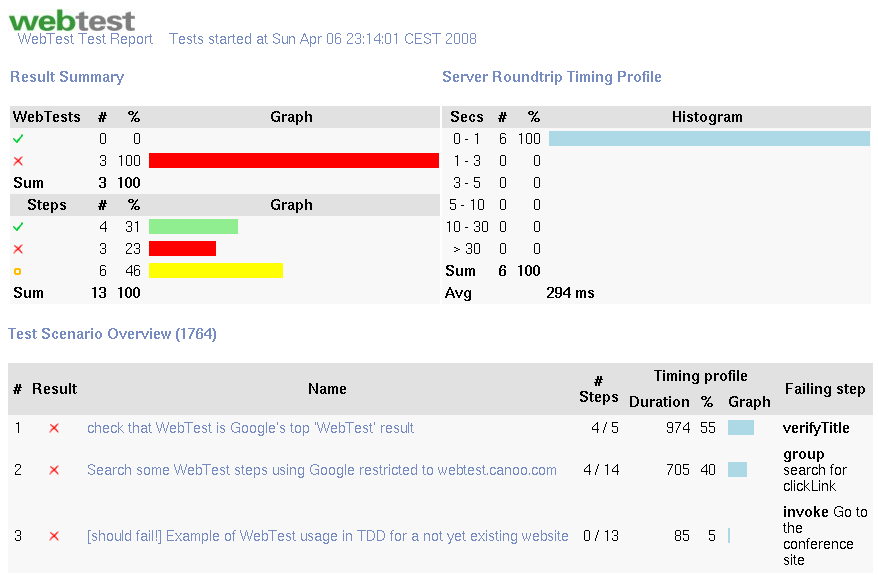
\includegraphics[width=0.8\linewidth]{qm/canoo-webtest-report}
  \caption{Canoo Webtest Report}
  \label{fig:canoo-webtest}
\end{figure}
Man kann Webtest auch in einem Maven-Projekt verwenden:
%allerdings muss zur Zeit das Plugin von Siegfrid Goeschl's Web-Seite
%
%\href{http://people.apache.org/~sgoeschl/download/maven-plugins/webtest-maven-plugin}
%  {people.apache.org/~sgoeschl/download/maven-plugins/webtest-maven-plugin}
%
%herunter geladen
% und eigenhändig im Maven-Repository installiert werden:
%
% Siehe:
% http://mguillem.wordpress.com/2009/04/30/webtest-with-groovy-maven-and-eclipse/
%
% ant -f /usr/local/java/webtest/webtest.xml wt.createProject
%
\begin{lstlisting}[language=xml,
  morekeywords={plugin,groupId,artifactId,configuration,host,port,haltonfailure,haltonerror,loglevel,executions,execution,phase,goals,goal}]
  <plugin>
    <groupId>org.codehaus.mojo</groupId>
    <artifactId>webtest-maven-plugin</artifactId>
    <configuration>
      <host>localhost</host>
      <port>8080</port>
    </configuration>
    <executions>
      <execution>
        <phase>integration-test</phase>
          <goals>
	    <goal>test</goal>
	  </goals>
	</execution>
      </executions>
  </plugin>
\end{lstlisting}
Das Plugin erwartet die webtest.xml-Datei im Verzeichnis
src/test/webtest.

Eine gutes Beispiel dazu findet man bei
Matt Raibles AppFuse-Framework \href{http://appfuse.org}{appfuse.org},
welches auch ganz allgemein beim Kick-Starting von Web-Projekten
ungemein nützlich ist.
%
% weitere beispiele:
%
% http://www.philliprhodes.com/content/testing-drupal-grails-webtest
% http://weblogs.java.net/blog/felipegaucho/archive/2009/11/18/testing-pdf-files-canoo-webtest-and-maven2
%
%
%\begin{lstlisting}[language=xml]
% <dependencies>
%     ...
%     <dependency>
%         <groupId>com.canoo.webtest</groupId>
%         <artifactId>webtest</artifactId>
%         <version>3.1-SNAPSHOT</version>
%     </dependency>
% </dependencies>
% ...
% <repositories>
%     <repository>
%         <id>webtest-dependencies-snapshot</id>
%         <name>WebTest dependencies</name>
%         <url>http://webtest.canoo.com/webtest/m2-repo-snapshots</url>
%     </repository>
% </repositories>
% \end{lstlisting}

\newslide
\subsubsection{Selenium}
Selenium ist ein OpenSource-Framework für Abnahme-, System und
Funktionstests von Web-Applikationen. Selenium kann auf
unterschiedliche Weise eingesetzt werden:
\begin{itemize}
\item in einem Browser: Selenium Core (unterschiedliche Browser)
  eventuell in Ergänzung mit Selenium IDE (Firefox)
\item als Proxy-Server: Selenium Remote Control (RC) für die Durchführung
  automatisierter Web-Tests in unterschiedlichen Programmiersprachen
  (Java, C\#, Perl, Python, Ruby)
\end{itemize}
\newslide
Beispielsweise in Kombination mit JUnit:
\begin{lstlisting}[language=java]
public class SeleniumWebTest extends TestCase {
  private DefaultSelenium selenium;

  public void setUp() throws Exception {
    super.setUp();
    selenium = new DefaultSelenium("localhost", 4444,
                                   "*firefox",
                                   "http://localhost:8080/");
    selenium.start();
  }

  public void tearDown() throws Exception {
    selenium.stop();
    super.tearDown();
  }

  public void testHelloWorld() throws Exception {
    try {
      selenium.open("http://localhost:8080/hitchhikers-guide");
      assertEquals("Hello World", selenium.getText("//h2"));
    } catch (SeleniumException ex) {
      fail(ex.getMessage());
      throw ex;
    }
  }
}
\end{lstlisting}
\newslide
In einem Maven-Projekt (genauer in einem von Maven verwalteten Projekt)
ergänzt man das POM-File mit dem folgenden Dependency-Element
\begin{lstlisting}[language=xml,
  morekeywords={dependency,groupId,artifactId,version,scope,enabled}]
<dependency>
   <groupId>
      org.openqa.selenium.client-drivers
   </groupId>
   <artifactId>selenium-java-client-driver</artifactId>
   <version>0.9.2</version>
   <scope>test</scope>
</dependency>
\end{lstlisting}
\newslide
Dazu wird ein spezielles Maven-Repository benötigt:
\begin{lstlisting}[language=xml,
  morekeywords={repositories,repository,id,name,url,layout,snapshots,releases}]
 <repositories>
        <repository>
            <id>openqa</id>
            <name>OpenQA Repository</name>
            <url>http://maven.openqa.org</url>
            <layout>default</layout>
            <snapshots>
                <enabled>false</enabled>
            </snapshots>
            <releases>
                <enabled>true</enabled>
            </releases>
        </repository>
  </repositories>
\end{lstlisting}
\newslide
sowie die beiden folgenden Plugins:
\begin{lstlisting}[language=xml,
  morekeywords={plugin,groupId,artifactId}]
<plugin>
 <groupId>org.codehaus.mojo</groupId>
 <artifactId>selenium-maven-plugin</artifactId>
</plugin>
<plugin>
  <groupId>org.mortbay.jetty</groupId>
  <artifactId>maven-jetty-plugin</artifactId>
</plugin>
\end{lstlisting}
\newslide
Nun kann in einem Terminal die Web-Applikation gestartet werden:
\begin{lstlisting}
  % mvn jetty:run
\end{lstlisting}
in einem zweiten Terminal der Selenium-Server:
\begin{lstlisting}
  % mvn selenium:start-server
\end{lstlisting}
und schliesslich in einem dritten Terminal der Test:
\begin{lstlisting}
  mvn test
\end{lstlisting}
Für weitere Vereinfachung siehe

\href{http://wiki.foochal.org/index.php/Maven_Selenium#Simple_selenium_java_unit_test}
{wiki.foochal.org/index.php/Maven\_Selenium\#Simple\_selenium\_java\_unit\_test}

und

\href{http://binil.wordpress.com/2006/12/08/automated-smoke-tests-with-selenium-cargo-testng-and-maven/}
{binil.wordpress.com/2006/12/08/automated-smoke-tests-with-selenium-cargo-testng-and-maven/}
%
\begin{figure}[H]
\begin{center}
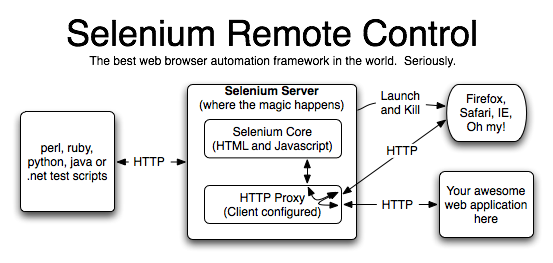
\includegraphics[width=\linewidth]{qm/selenium-rc}
\end{center}
\caption{Selenium Remote Control
  (Quelle \href{http://www.openqa.org/selenium-rc/tutorial.html}
   {www.openqa.org/selenium-rc/tutorial.html})}
\end{figure}
\begin{figure}[H]
\begin{center}
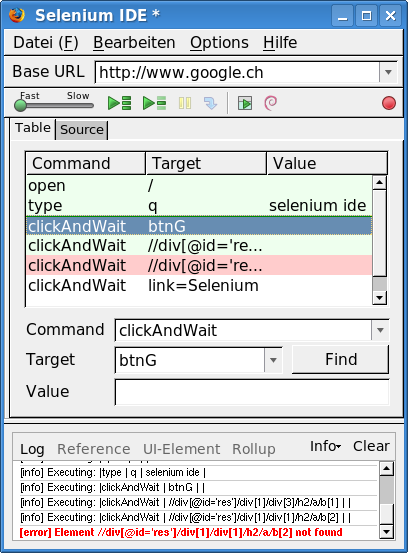
\includegraphics[width=0.5\linewidth]{qm/selenium-ide}
\end{center}
\caption{Selenium IDE als Firefox Plugin}
\end{figure}
%

%\subsection{Software und weitere Informationen}
%%% Local Variables:
%%% mode: latex
%%% TeX-master: "projektskizzen"
%%% End:
